\documentclass[a4paper]{article}

\usepackage[portuges,english]{babel}
\usepackage[latin1]{inputenc}
\usepackage{fancyvrb}
\usepackage{graphicx}
\usepackage[a4paper,left=20mm,right=20mm,bottom=20mm,top=15mm]{geometry}
\usepackage{moreverb}
\usepackage{amsthm}
\usepackage{listings}


\title{Precomputing Avatar Behaviour From Human Motion Data}

\date{\today}

\newtheorem{constr}{CONSTRAINT}

\author{
Nuno A. Silva\\ \small pg17455@alunos.uminho.pt \\ Universidade do Minho
\and
Luis Miranda\\ \small pg14439@alunos.uminho.pt \\ Universidade do Minho
}

\begin{document}

\maketitle

%\abstract


%%%%%%%%%%%%%%%%%%%%%%%%%%
\section{Introduction}
%%%%%%%%%%%%%%%%%%%%%%%%%%
This report refers to a work based on a paper from Lucas Kovar, et. al\ref{motiongraphs}, particularly the path synthesis technique described there. Motion Graphs is a method for creating realistic, controllable motion. In Kovar's work a directed graph is automatically generated, this graph contains pieces of original motion and automatically generated transitions. The authors also presented a general framework for extracting a particular graph walk that meet the user's specifications, and apply this framework to a specific problem with different styles of locomotion and arbitrary paths. \\

Path synthesis relates to this final step in the proposed framework, where a user specifies a path and a graph walk is performed in order to generate the locomotion that best suits the path. The goal is to integrate this specific module into a larger virtual character locomotion system. Ideally the user defined path should be aproximated by a spline and then a search in the motion graph should be done in order to find a set of motion capture data that minimizes the error. This error is the sum of the squared differences between the defined path and the path that the animation will produce, for that it is used the arc-length distance of the paths. \\

The OGRE engine will be used as the basis for the entire project. A scene with a model is generated where the user can input the desired path to traverse. Once the program finds the set of motions that respect the rules explained above, it is rendered on the scene.



%%%%%%%%%%%%%%%%%%%%%%%%%%
\section{Implementation details}
%%%%%%%%%%%%%%%%%%%%%%%%%%
The implementation can be divided in three  different parts, step one, where the user define the path, step two, were the animations are chosen and step three, where the animation that follows the user path is showed. Each one is a fundamental operation off the whole system. The whole process works as one can see on the following workflow on picture ~\ref{fig:work}.
\\
\begin{figure}[hbtp]
\begin{center}
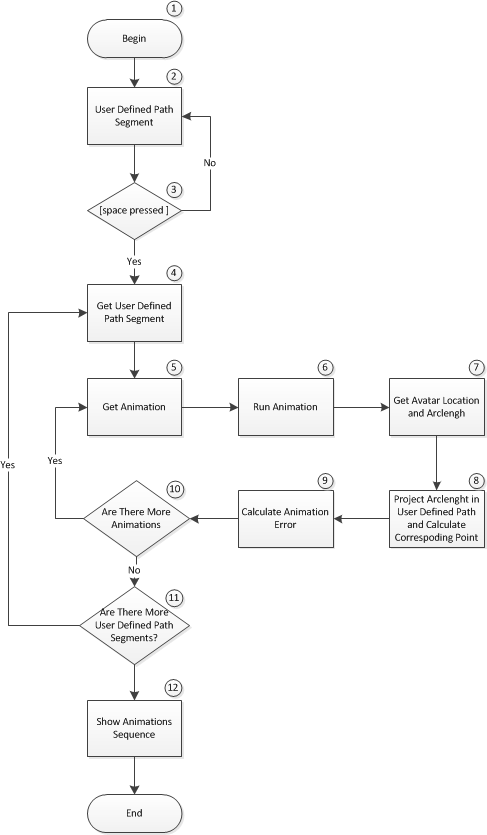
\includegraphics[scale=0.8]{Images/fluxograma.png} 
\caption{\textit{Workflow}}
\label{fig:work}
\end{center}
\end{figure}

User path definition (step 1 in picture ~\ref{fig:work}) is the step where the user defines a simple path which the avatar would ideally travel.   The user defined path is a sequence of vectors between points chosen by the user in the application screen (picture ~\ref{fig:uapath}). The user, using the mouse, can define a set of points in a plane. This points will be used in the construction of a line that passes trough them. Ideally this line should be a spline (picture ~\ref{fig:uapath}), but in the current state, our work only supports a straight path between each pair of points. 
\\
\begin{figure}[hbtp]
\begin{center}
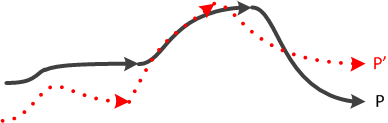
\includegraphics[scale=0.8]{Images/UserPathVSAvatarPath.png} 
\caption{\textit{User defined path(bold line) and avatar path(dot line)}}
\label{fig:uapath}
\end{center}
\end{figure}

In picture ~\ref{fig:uapath}, one can see as example, in bold, the user defined path, and in dot line a path that an avatar could in effectively follow.  
\\

After the path is defined, the user can press the space key (step 3 in picture ~\ref{fig:work}), so the next phase, where the animations are evaluated for error, starts.
\\

To make an animation that runs along the path defined by the user, a set of animations from motion capture data must be chosen.  However, not all animations are suitable to fit in a path defined by the user. This arises the question, how to choose animations that fit the path defined by the user? The answer to this question is to associate to each animation, an error. This error will depend of the path followed by the animation, and it will be great if the animation deviates largely from the user defined path and smaller, if the animation, follows a path that is similar to the one defined by the user. 
\\
\begin{figure}[hbtp]
\begin{center}
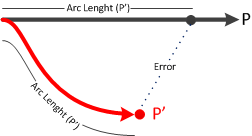
\includegraphics[scale=0.8]{Images/error.png} 
\caption{\textit{Error definition}}
\label{fig:error}
\end{center}
\end{figure}

First a segment from the path P defined by the user is selected. For this segment, before the error can be calculated, the software must load and display the animations, so the path travelled by each one of them can be measured. This operation is done following Ogre\textquoteright s method for displaying animations. To start, all the animations available for the current avatar are loaded. Then, for each one of this animation, we start by running it (P\textquoteright on figure ~\ref{fig:error}). After the animation reaches the end, we can start to calculate the error (steps 8, 9 and 9 in figure ~\ref{fig:error}). The error can be defined as the distance between the arclength of the point where the animation ends, in the animation path (P\textquoteright) and the point at the same arclength in the user defined path (P).  
\\

We start by projecting the arclength of P\textquoteright in P, so we can discover the point in P that corresponds to the point with the same arclength of the endpoint in P\textquoteright. From this, the arclength is smaller than the path P or greater than the path P.  If the arclength is smaller, one can simple calculate the point recurring to the parametric equation of a line in 3D space.  If the arclength is greater than the length of P , the error is calculated using the end point of P. 
\\

We then choose the animation with a smaller error, which is the one that will follow a path similar to the one defined by the user. 
\\

After this, the process is repeated for all animations in each segment of the user defined path. 






%%%%%%%%%%%%%%%%%%%%%%%%%%
\section{Conclusion and future work}
%%%%%%%%%%%%%%%%%%%%%%%%%%
The implementation can still improve in many ways. For a start, the correct display of the calculated motion. Also splines should be used for the user defined path. Aditionally, it would be good to improve the user interaction with the program, and finally fully integrate it with the remaining system.





%%%%%%%%%%%%%%%%%%%%%%%%%%
\begin{thebibliography}{}

\bibitem{motiongraphs}
{Lucas Kovar, Michael Gleicher and Frederic Pighin},{Motion Graphs}, {2002}
    
    
\end{thebibliography} 


\end{document}
